\documentclass{article}
\usepackage[dvips]{graphicx}
\author{David J. Burger}
\title{The Messaging Library}
\begin{document}
\maketitle

There is a saying in computer lore that says "every program expands
until it has the ability to send and receive email."  In the LILT lab,
this saying might evolve to "every program expands until it provides
the ability to do distributed collaboration."  For desktop
applications, this means providing a system for sending messages to
either a centralized server or peers over the Internet.  Programming
ad hoc messaging solutions for every application leads to a lot of
unnecessary duplication of effort.  In this paper I will describe the
light weight, event based, extensible messaging library I have written
that can serve the messaging needs of applications written in the LILT
lab.  In doing so I will answer the four main questions that guided
the design of the messaging library:

\begin{enumerate}
\item What types of messages should the messaging library handle?
\item How should messages be delivered from the library to the
      application using the library?
\item What types of connections should the messaging library work
      over?
\item How should the object hierarchy of the messaging library be
      designed?
\end{enumerate}

I will also mention the reference implementations used to test the
messaging library.

An addendum has been added to this paper which details modifications
made to the messaging library in response to its usage as the
communications system for the House Party project.  The addendum also
includes empirical results which compare the efficiency of the
messaging library when operating with various connection and message
types.  At the end of the paper you will find sample source code that
shows how to use the library as well as the UML diagrams of the key
components of the library.

\section{What types of messages should the messaging library handle?}

Before writing a messaging library one needs to ask what type of
messages applications will need to exchange.  The types available
need to be general enough for all programs to use the
library and yet specific enough to allow programs to communicate with
a convenient message type.  The three types of messages that
cover the range that Java applications need are Java
serializable objects, Java XML Documents in text form, and pure text
messaging.

Using Java serializable objects is considered a quick and dirty way
to provide a messaging protocol in Java networked applications.
It is quick both in terms of implementation time and execution time.
Quick implementation is facilitated by subclasses of the stream
classes within the Java class libraries that know how to read and
write Java objects.  The execution time of messaging libraries using
Java objects should also be very fast since a compact  native binary format is
used to send the data.  Using Java
objects is considered dirty because changing an object's
implementation can render it incompatible with previous
versions of the same object [Bloch, Effective Java, p. 213].  This has
grave implications for data stored in an older object format and for
distributed clients that must be upgraded to the new object format at
the same time.  Another drawback to using Java objects for messaging
is that it will practically mandate that your entire system be written
in Java.

Using XML as a messaging protocol avoids several of the problems that
exist when using Java objects.  XML, being a simple but flexible text
format, is ideal for exchanging data with heterogeneous systems.
Designing the XML format for application specific messages will
involve more effort but the resulting system won't be susceptible to
the change of implementation problem that Java objects have.
Drawbacks to using XML are an increased message size given XML's
verbose format and the processing time needed to parse XML documents.
Both of these problems will result in a reduced message
exchange speed.

Pure text messaging involves sending raw text in a custom format.
This type of messaging can be used when the communication needs
of an application are very simple.

For the messaging library I chose to provide the ability to send Java
serializable objects and XML documents as messaging protocols.  Because
of the problems associated with implementation changes in Java objects
it is unlikely that we will be using Java objects as the messaging
protocol for any LILT applications.  However, this
functionality is good for a quick demonstration implementation or to
gradually migrate an existing application into a networked application.
Pure text messaging has not been implemented but the existing
messaging library could be easily extended to support it.  Later in
this paper I will explain a design pattern that has been used to
develop the messaging library which makes such an extension quite
easy.

\section{How should messages be delivered from the library to the application using the library?}

Another design decision that must be made in the design of a messaging
library is the manner of the delivery of messages from the library to
the application using the library.  The initial connection made by a
client application is likely to include a handshake of some sort that
contains, for example, authentication information.  In this type of
situation a blocking read is helpful because the application can't
proceed until the handshake is complete.  Therefore the messaging
library provides blocking reads and writes through implementers of
the Messenger interface and the readMessage and writeMessage method
calls.  After the handshake, most applications will need asynchronous
reads as information is processed for the local client while waiting
for any activity over the communications channel.  While each
individual application could use a specific implementation of the
Messenger interface along with a Thread to design an asynchronous read
strategy, this would introduce a lot of duplicate effort for each
application.  Therefore asynchronous reads are handled by the
messaging library by constructing a MessengerThread object with an
instance of the Messenger class.  The MessengerThread class handles
asynchronous reads with a thread that repeatedly calls the
Messenger's readMessage method.

Clients wishing to accept received messages must implement the
MessageListener interface and then register with the
MessengerThread class through the addMessageListener call.  When a
message is received it is delivered to all the registered listeners
through a messageReceived(MessageEvent) callback.  Clients also need
to be concerned about Exceptions that may occur while the
MessengerThread is reading messages.  In most cases Exceptions will be
considered fatal, and the client will need to shut down the
MessengerThread to avoid an infinite loop of exceptions.  Similar to
asynchronous message delivery, exceptions are handled by clients
implementing the ExceptionListener interface and then registering
themselves with the MessengerThread through the addExceptionListener
method.  Any exceptions that occur are delivered to the client via an
exceptionThrown(ExceptionEvent) callback.

The asynchronous message and exception delivery methods described
above are modeled after the event system for GUI events in the Java
Swing libraries.  This design pattern is known as the event listener
pattern (also the Observer-Observable pattern or Publisher-Subscriber
patterns).  The real advantage of this system is the loose coupling it
provides where the MessengerThread does not know who is listening to
the events it provides.  Instead, it merely maintains lists of
objects that implement the MessageListener and ExceptionListener
interfaces that will be notified when the corresponding events occur.

\section{What types of connections should the messaging library work over?}

Another major design decision that must be made in the design of a
messaging library is what type of network connection to use for the
network transport.  The obvious and easiest answer to that question is
to use a simple socket.  Unfortunately in the real world the presence
of firewalls severely limits the usability of a socket only
messaging library.  Schools in particular are likely to have
restrictive firewalls in place.  Firewalls may be configured to only
accept traffic from the well known HTTP port 80.  More sophisticated
firewalls may even inspect network packets disallowing any traffic
that isn't HTTP.  With these restrictions in place, it becomes clear
that the messaging library needs to be able to tunnel its messages
within an HTTP connection.

HTTP operates on what is called a request-response paradigm.  With the
original specification this means that a client generates a
request for information, and sends it to the server.  The server
responds to the request and then close the connection.  Each subsequent
request is sent with a new connection.  Building up and tearing down
each individual connection results in a lot of overhead.  HTTP
version 1.0 introduced an unofficial Keep-Alive header that would
allow the client to make more than one request on the same
connection.  HTTP version 1.1 made all connections Keep-Alive unless
the client stated it wanted otherwise with a "Connection: close"
header.  Even with HTTP version 1.1, there is no guarantee that the
client or server will actually keep the connection open, therefore it
is not something you can write an application to rely upon.  This
makes it necessary to develop the messaging library with the worst
case scenario in mind, that is making a new connection for each
request [Jim Driscoll, HTTP Keep Alive,
http://www.io.com/$\sim$maus/HttpKeepAlive.html].
This requires including data with each request that will
allow the server to identify the connection.

For the messaging library the manner in which extra data is included
to identify the connection is dependent on the type of data being
transmitted.  With an Object messenger the data is encapsulated within
an ObjectEnvelope object.  The ObjectEnvelope class maintains a
reference to the enclosed Object as well as to a connection identifier
string.  When sending XML the messaging library will add a
"connectionId" attribute to the root element of the XML document being
transmitted.  Servers that work with the messaging library must supply
these identifiers during the initial connection handshake.  For an
Object messenger, the request for an identifier is indicated by a new
connection that sends a null object.  The server is expected to
respond with a String identifier.  For an XML messenger, the request
for an identifier is indicated by a new connection that sends a
"$<$hello /$>$" document.  The server is expected to respond with a
"$<$hello connectionId="the id" /$>$" response.  In either case the
application developer is completely shielded from these transactions
and can use the messaging library exactly as if it were using a simple
socket for message transport.  Reference versions of servers that
perform the connection handshakes for HTTP messaging are described
below.

It is beneficial to the application developer to strive for Keep-Alive
connections when possible as this will result in a quicker messaging
system.  The messaging library uses the HttpUrlConnection from the Java
class libraries to make connections to HTTP servers.  The usage of
this library provides two key benefits.  The first benefit is in the
simplification of the code that uses HTTP as a transport mechanism.
The HttpURLConnection class has methods for making the connection and
setting the various headers needed by the messaging library.  The
second benefit is that Keep-Alive requests are handled internally by
the library with a cache of client connections.  This frees the
messaging library implementation from the problem of getting
Keep-Alive connections and then recovering when such a connection gets
dropped.

\section{How should the object hierarchy of the messaging library be designed?}

The final hurdle in developing the messaging library was designing the
Object hierarchy to follow the programming principle "don't repeat
yourself."  The original design of the messaging library had an object
hierarchy as seen in Figure~\ref{old}

\begin{figure}[!hbp]
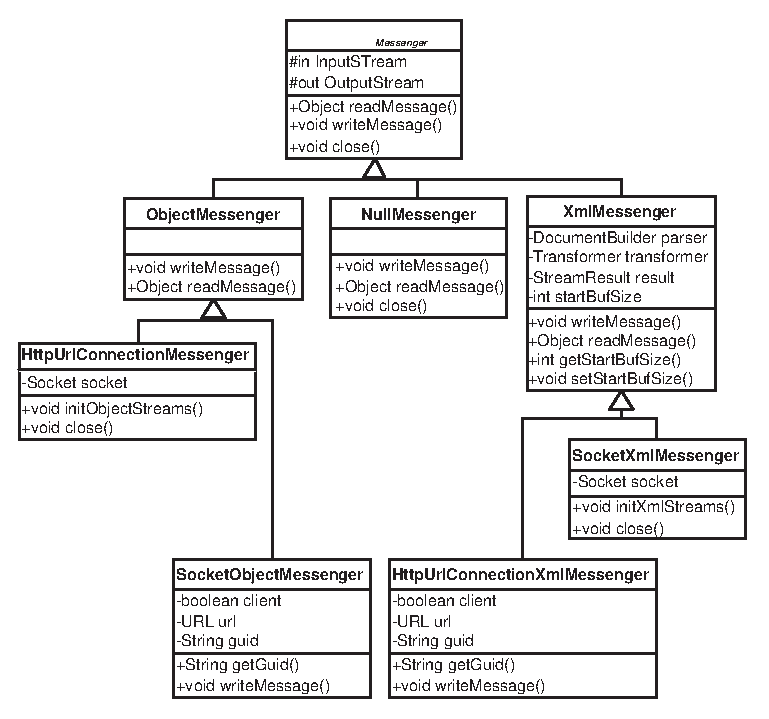
\includegraphics{old.eps}
\caption{The original messaging library.} \label{old}
\end{figure}

The obvious problem with the design is that the two types of
messengers that extend the Messenger class, Object and XML, need to
have the ability to operate over both HTTP and sockets.  This results
in the repetition of socket code and HTTP code in
both branches of the Object hierarchy above.  This type of repeated
code is more difficult to maintain and extend.  For example, if it were
discovered that the setting of an additional header would improve the
performance of an HTTP connection then the same change would need to be
made in both branches of the Object hierarchy.  Even worse, the
introduction of a new type of Messenger, say a TextMessenger, would
require the introduction of three new classes with even more repeated
code.

The solution to this problem was to use the strategy design pattern
[Gamma, Helm, Johnson, Vlissides, Design Patterns, p. 315].
A strategy pattern provides a way to configure a class with one of
many behaviors.  For the messaging library, the behavior that needs
variation is operations that are performed on the streams that are
used during messaging.  These operations include initialization,
sending data, receiving data, tagging data with a connection
identifier, and reading a returned connection identifier.

The first step necessary to refactor the original design into a
strategy approach was to change the Messenger class into an interface
with methods to send and receive messages.  The NullMessenger class
and the StreamMessenger class implement the Messenger interface.  The
NullMessenger is a class that doesn't actually send or receive any
messages.  This class is extremely useful when set as the Messenger
for a distributive application working in standalone mode.  The
StreamMessenger abstract class incorporates the strategy pattern by
holding a reference to a class that implements the StreamStrategy
interface.  Implementing the StreamStrategy interface requires
implementing methods that take a stream object as a parameter and
perform initialization, sending messages, reading messages, and adding
a connection identifier.  The concrete subclasses of the
StreamMessenger class are SocketMessenger and HttpURLConnection
messenger.  These classes know how to make socket and HTTP connections
as the class name indicates, thus establishing the streams needed for
communications.  Both classes take a StreamStrategy object in their
constructors and forward any needed stream operations to the concrete
StreamStrategy that they were constructed with.  Currently two
StreamStrategy concrete subclasses exist, ObjectStreamStrategy and
XmlStreamStrategy.  ObjectStreamStrategy knows how to send and receive
Java objects over streams while XMLStreamStrategy does the same for
XML documents by converting them into text.  The major benefits of
this design can be easily seen when one considers what it would take to
add pure text messaging capability to the messaging library.  With the
strategy pattern it would only take a TextStreamStrategy
implementation of the StreamStrategy interface.  This is a great
reduction in the amount of effort and duplicated code necessary to
extend the library compared to the effort for the old design as
described above.

\section{Reference Implementations}

In developing the messaging library several reference implementations
have been made to exercise the various capabilities of the library.
These include the following programs:

\begin{itemize}

\item SampleBroadcastServer.java - a socket based server that accepts
connections from clients using the messaging library with a
SocketMessenger.  All received messages are forwarded to all connected
peers.  When executed command line parameters can be provided to
operate the server in either Object or XML mode.  This program resides
within the CVS repository for the messaging library.

\item SampleChatServer.java - similar to the SampleBroadCastServer, but
provides greater feedback on the messages as they travel through the
server.  This program resides within the CVS repository for the messaging
library.

\item SampleChatClient.java - a socket based chat client that can
communicate using sockets or HTTP connections.  It will thus
inter-operate with the SampleBroadCastServer and SampleChatServer
described above as well as through HTTP connections to the reference
servlet implementations described below.  Command line parameters
control its runtime options, that is Object or XML, and socket or
HTTP.  This program resides within the CVS repository for the messaging
library.

\item SampleMySqlBroadcastServer.java - a socket based server similar to the
SampleBroadCastServer that logs all messages to a MySQL database.
When new clients connect to the server they are immediately forwarded
all previously logged messages.  This server can only operate in XML
mode as it stores the text of the XML messages to the database.
Object operation could be facilitated by storing the data to binary
MySQL data fields.  This program resides within the CVS repository for the
messaging library.

\item ObjectServlet.java - acts as a broadcast server of Object messages
over HTTP.  It also provides a simple example of handling the
handshake needed to maintain state over the HTTP connection when using
Object messaging.  This program resides within the sampleservlets CVS
repository.

\item XmlServlet.java - acts as a broadcast server of XML messages over
HTTP.  It also provides a a simple example of handling the handshake
needed to maintain state over the HTTP connection when using XML
messaging.  This program resides within the sampleservlets CVS
repository.

\item Discuss - a simple threaded discussion client that can connect to the
SampleBroadcastServer and SampleMySqlBroadcastServer described above.

\end{itemize}

\section{Addendum}

Shortly after completing the messaging library it was put to work as the
underlying messaging system for the House Party application framework.  This
was an opportunity to test the design of the system and make changes where
necessary.  This document addresses the changes that have been made to the
messaging library from the House Party experience.  It also includes empirical
data concerning the speed of message exchange with the various message and
connection types.

One addition that was necessary was to create a new StreamStrategy that
handles JDOM Document objects directly.  During the creation of the messaging
library I attempted to avoid dependencies on libraries that aren't available
in the default Java SDK.  This caused me to use the basic org.w3c.dom
interfaces and default implementations for the XML portions of the messaging
library.  Many people in the Java community choose to use JDOM because of its
more object oriented interface.  House Party is one such application that uses
JDOM internally for the creation of XML that represents the various entities in
the program  While it is simple to convert org.jdom.Document objects to
org.w3c.dom.Document objects and vice versa, it becomes a processing
step that must take place before and after every message transmission in the
House Party system.

Because the original design of the messaging library used a strategy
design pattern for the transmission of data over streams this step was
quite simple.  It was accomplished by changing the current
XmlStreamStrategy into a W3cDomStreamStrategy and adding a
JdomStreamStrategy.  The work involved also involved factoring out
some of the common XML processing into an abstract class called
XmlStreamStrategy .  The only hitch involved in the implementation was
the discovery that the JDOM parser doesn't appreciate being fed white
space between document transmissions.

The second addition that was necessary was caused by the need to delay message
arrival in the House Party system to facilitate testing.  This would allow
synchronous and asynchronous situations to be disguised to achieve a certain
effect, such as making a largely synchronous test trial appear to occur
asynchronously.  With this need in mind I created the BufferedMessenger
and BufferedMessengerThread classes.  The BufferedMessenger class provides
the ability to add buffering to any Messenger in a synchronous messaging
environment.  The BufferedMessengerThread class provides the ability to have
buffered asynchronous messaging delivery with any Messenger class.
The number of messages to buffer can be changed with calls to
setInBufSize(int) and setOutBufSize(int).  The methods flushReads()
and flushWrites() can be used to clear the buffers at any time.  While
a BufferedMessengerThread can be constructed with a BufferedMessenger
it will result in ``double buffering'' and is certainly not
recommended.

The BufferedMessenger uses a design pattern called the Decorator pattern
[Gamma, Helm, Johnson, Vlissides, Design Patterns, p. 175].  The decorator
pattern allows a new class to add behaviors to an existing class.  This is
achieved by the decorator implementing the same interface as the class it will
decorate.  By sharing the same interface, the decorator can be used
transparently as the decorated class.  When constructed, the decorator is
supplied a reference to the object it will decorate.  When a method of the
decorator is called it can ``decorate'' the call by adding extra behaviors
before and after forwarding the call to the decorated object.  In the case of
the BufferedMessenger, this allows for a check against the associated buffer
size before actually sending or receiving the message.

The messaging library now contains code that takes advantage of two
design patterns, strategy and decorator.  The strategy pattern is seen
as a way of modifying the ``guts'' of a class and is used to vary the
method by which data is sent over streams.  The decorator pattern is
seen as a way of changing the ``skin'' of a class and is used to
provide message buffering around read and write calls.

Sample client programs have been added that exercise the new features
of the messaging library.  Test runs have been made to ensure that a
client using a W3cDomStreamStrategy can interoperate with a client
using a client using JdomStreamStrategy as only raw XML text is
transmitted.  The Discuss application, a test bed for the House Party
framework, was also briefly modified to test the new buffered
messenger classes adding buttons to flush reads and writes.

When using the messaging library a decision must be made whether to use XML
message types or Java Object serialization.  Several advantages come from using
the messaging library with XML messages compared to using Java Object
serialization.  The most obvious advantage is the avoidance of the problem
associated with Object incompatibilities that  occur as the Object's being
passed via the library evolve.  A second is that with XML is is easy to mix
components written in Java with components written in other languages.  While
these advantages are compelling, it was interesting to look at the decrease in
message exchange rate that comes from using XML instead of Java Object
serialization.

To test the speed difference I wrote a program called SampleRttTester.  The
RTT stands for ``round trip time.''  SampleRttTester is capable of making both
socket and HTTP connections.  When launched, command line parameters determine
if it sends objects, W3C DOM generated XML, or JDOM generated XML.  The final
command line parameter indicates how many messages it should send.  I ran the
program against the SampleBroadcastServer for socket connections and sample
servlets for HTTP connections.  SampleRttTester records a time stamp upon
starting and then send the appropriate number of messages.  Upon receipt of
each message a counter is decremented.  When the counter reaches zero a time
stamp is taken again and the difference is noted.

In Table 1 below you will find the results of running the
SampleRttTester.  The test environment consisted of two computers
connected through a 10 MB hub on a local area network.  The client
computer was a Macintosh running OS X with a G3 processor while the
server was an Intel Pentium III machine running Linux.  Each test
trial was ran ten times to produce an average result.  Every test
involved the sending of 1000 identical messages.  As expected, Java
Object serialization proved to be much faster than XML messaging.
When used with a socket it was more than five times faster than XML
messaging.  Surprisingly, XML messaging using the W3C DOM interfaces
was more than 1.5 times as fast as XML messaging with JDOM.

The tests also demonstrated the large overhead associated with using HTTP
connections with the messaging library.  Java Object serialization was 7.5
times slower using an HTTP connection than when using an ordinary socket.  The
XML messaging types showed similar slowdowns.  Even with the obvious cost of
HTTP messaging, its utility for allowing messaging through firewalls is a major
redeeming quality.

\begin{table}[!hbp]
\centering
\begin{tabular}{|c|c|c|c|}
\hline
\multicolumn{4}{|c|}{RTT 1000 Messages (milliseconds)} \\
\hline
 & Object & W3C DOM & JDOM \\
\hline
RTT Socket & 452.7 & 2315.1 & 3910.2 \\
\hline
RTT HTTP & 3403.5 & 10681.2 & 13154.7 \\
\hline
\end{tabular}
\caption{Messaging Library Round Trip Time Tests}
\end{table}

\section{Sample Source Code}

\begin{verbatim}
// current concrete strategies are ObjectStreamStrategy
// and XmlStreamStrategy
Strategy strategy = new XmlStreamStrategy();

// current concrete messengers are HttpUrlConnectionMessenger,
// NullMessenger, and SocketMessenger
Messenger messenger =
    new HttpUrlConnectionMessenger(server, strategy);

// the messenger thread provides asynchronous reads of messages
// and exceptions with event type delivery
MessengerThread messengerThread = new MessengerThread(messenger);

// connecting the listeners
messengerThread.addMessageListener(messageListener);
messengerThread.addExceptionListener(exceptionListener);

// this will cause the read loop to start
messengerThread.start();

// sending a message
messengerThread.writeMessage(message);
\end{verbatim}

\section{UML Diagrams}

\begin{figure}[!hbp]
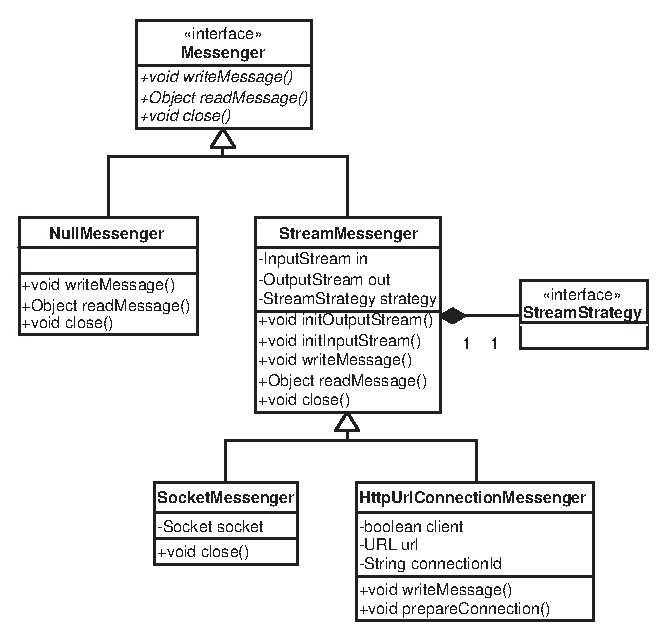
\includegraphics{new.eps}
\caption{The core of the messaging library.} \label{new}
\end{figure}


\begin{figure}[!hbp]
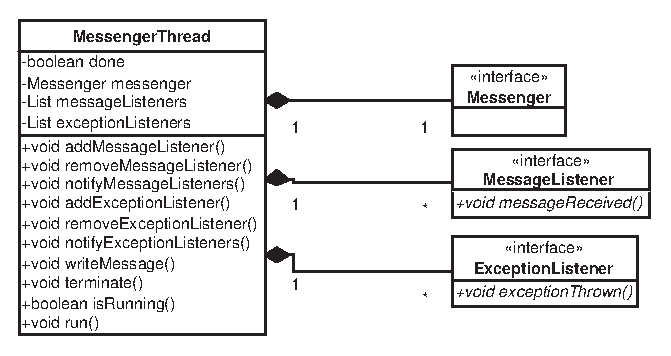
\includegraphics{mess.eps}
\caption{The MessengerThread provides asynchronous delivery.} \label{mess}
\end{figure}


\begin{figure}[!hbp]
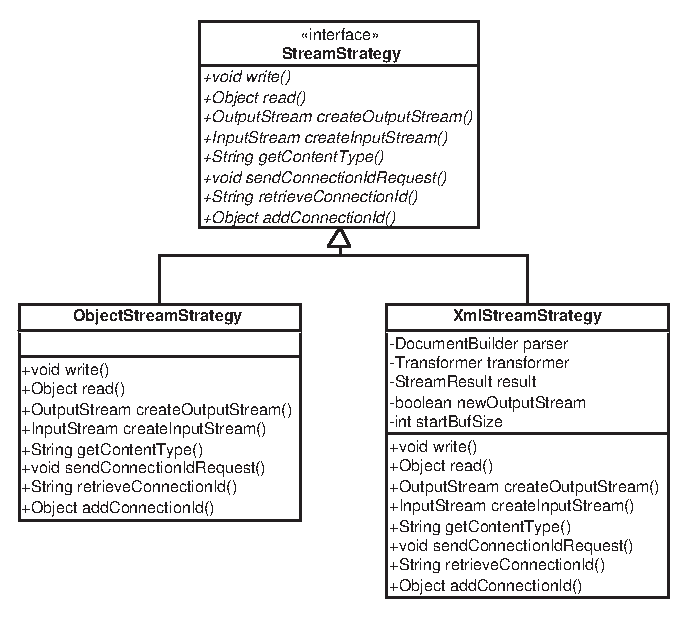
\includegraphics{strat.eps}
\caption{The StreamStrategy classes.} \label{strat}
\end{figure}

\end{document}
